\documentclass[10pt,pdf,hyperref={unicode}]{beamer}

% \usepackage{lmodern}
\usepackage[normalem]{ulem}
\usepackage{qrcode}
\usepackage{array}
\usepackage[T2A]{fontenc}
\usepackage[utf8]{inputenc}
\usepackage{colortbl}
\usepackage{listings}

% отключить клавиши навигации
\setbeamertemplate{navigation symbols}{}

% тема оформления
% все темы тут http://ccd.uab.es/~iblanes/beamer_gallery/index_by_theme.html
\usetheme{default}

\title{Семинар 2+3: целые числа и ввод-вывод}
\date{19 Ноября, 2019}


\begin{document}

% титульный слайд
\begin{frame}
  \titlepage
\end{frame}

\begin{frame}{Беззнаковые числа}
    \begin{itemize}
        \item Представляют из себя $N$-битные положительные целые числа на отрезке $[0, 2^N - 1]$
        \item Переполнение точно определено стандартом C (как сложение в $\mathbb{Z}_{2^N}$)
        \item $1111 + 0001 = \textcolor{red}{1}0000 = 0$
    \end{itemize}
\end{frame}

\begin{frame}
    \begin{center}
        \large{Как представлять отрицательные числа?}
    \end{center}
\end{frame}

\begin{frame}{Signed magnitude representation}
    \begin{itemize}
        \item Most significant bit (MSB) отвечает за знак: $0001 = +1$, $1001 = -1$
        \item Диапазон: $[-2^N+1, 2^N-1]$
        \onslide<2->\item Требуются отдельные операции сложения, вычитания и умножения для знаковых чисел
        \onslide<2->\item Два представления для 0: $0000 = +0$ и $1000 = -0$
    \end{itemize}
\end{frame}

\begin{frame}{One's complement}
    \begin{itemize}
        \item $-A = BitwiseNot(A)$
        \item Диапазон: $[-2^N+1, 2^N-1]$
    \end{itemize}
\end{frame}

\begin{frame}{One's complement}
    \begin{center}
        \onslide<1->{$-1 = 1110$} \\
        \onslide<1->{$+2 = 0010$} \\
        \onslide<2->$1110 + 0010 = \textcolor{red}10000 = 0$ \\
        \onslide<3->Упс...
    \end{center}
\end{frame}

\begin{frame}{One's complement: end-around-carry}
    \center{$1110 + 0010 = \textcolor{red}10000 = 0 + \textcolor{red}1 = 1$}
\end{frame}

\begin{frame}{One's complement: недостатки}
    \begin{itemize}
        \item Два представления для 0: $0000 = +0$ и $1111 = -0$.
        \item End-around-carry
        \item Зато сложение и вычитание одинаковое для знаковых и беззнаковых!
    \end{itemize}
\end{frame}

\begin{frame}{Two's complement}
    \begin{itemize}
        \onslide<1->\item Определение отрицательных чисел: $A + (-A) = 0$
        \onslide<2->\item Давайте каждому положительному числу сопоставим отрицательное
        \onslide<3->\item $-A = BitwiseNot(A) + 1$
        \onslide<4->\item Используется в современных процессорах
        \onslide<4->\item Одно представление нуля: $-0 = BitwiseNot(A) + 1 = 1111 + 1 = 0000 = +0$
        \onslide<4->\item Диапазон чуть больше: $[-2^N, 2^N-1]$
    \end{itemize}
\end{frame}

\begin{frame}{Two's complement: недостатки}
    \begin{itemize}
        \item Операции сравнения теперь сложные
        \item Умножение требует sign extension: 0010 = 00000010, 1000 = 11111000
        \item «Перекос» диапазона представимых чисел
        \onslide<2->\item abs(INT\_MIN) = ???
    \end{itemize}
\end{frame}

\begin{frame}{ZigZag representation}
    \begin{itemize}
        \item LSB кодирует знак числа
        \item $(A << 1) \mathbin{\oplus} (A >> 31)$
        \item Note that the second shift -- the \lstinline{(A >> 31)} part -- is an arithmetic shift. So, in other words, the result of the shift is either a number that is all zero bits (if A is positive) or all one bits (if A is negative)
        \item Одно представление нуля
        \item $-1 = 1111 \mathbin{\oplus} (1111 << 1) = 1111 \mathbin{\oplus} 1110 = 0001$
        \item $1 = 0000 \mathbin{\oplus} (0001 << 1) = 0000 \mathbin{\oplus} 0010 = 0010$
    \end{itemize}
\end{frame}

\begin{frame}{ZigZag representation}
    \begin{itemize}
        \item Вместе с varint-кодировкой экономит размер числа -- не нужно хранить ведущие нули
        \item Используется в Google Protocol Buffers
    \end{itemize}

    \begin{center}
    \qrcode[hyperlink,height=75px]{https://developers.google.com/protocol-buffers/docs/encoding\#signed-integers}
    \end{center}
\end{frame}

\begin{frame}
    \begin{center}
        \large{Целые числа в C}
    \end{center}
\end{frame}

\begin{frame}{Целые числа в C: типы данных}
    \begin{itemize}
        \item Знаковые типы: short, int, long, ...
        \item Тоже знаковые типы: signed char, signed short, signed int, ...
        \item Беззнаковые типы: unsigned char, unsigned short, ...
    \end{itemize}
\end{frame}

\begin{frame}{Целые числа в C: типы фиксированных размеров}
    \begin{itemize}
        \item Для каждого типа есть гарантии на диапазон, которое оно включает
        \item Но может включать больше!
        \item Типы фиксированного размера: int8\_t, uint16\_t, int32\_t, uint64\_t, ...
        \item Объявлены в inttypes.h
        \item Не работают, если платформа не поддерживает соотв. типы
    \end{itemize}
\end{frame}

\begin{frame}{Целые числа в C: немного мемов}
    \begin{itemize}
        \onslide<1->\item \textbf{char} читается как... \onslide<2-> ['kar]
        \onslide<3->\item \textbf{CHAR\_BIT} — количество бит в байте
        \onslide<4->\item Знаковость char... \onslide<5->\textbf{implementation defined}
        \onslide<6->\item long вмещает числа из $[-2^{32}, 2^{32}-1]$
    \end{itemize}
\end{frame}

\begin{frame}{Целые числа в C: про переполнение}
    \begin{itemize}
        \onslide<1->\item Переполнение signed-типов = \textbf{undefined behavior}!
        \onslide<2->\item Иногда нужно проверить, было ли переполнение, но без UB
        \onslide<3->\item Семейство функций \_\_builtin\_add\_overflow
    \end{itemize}

    \onslide<3->\center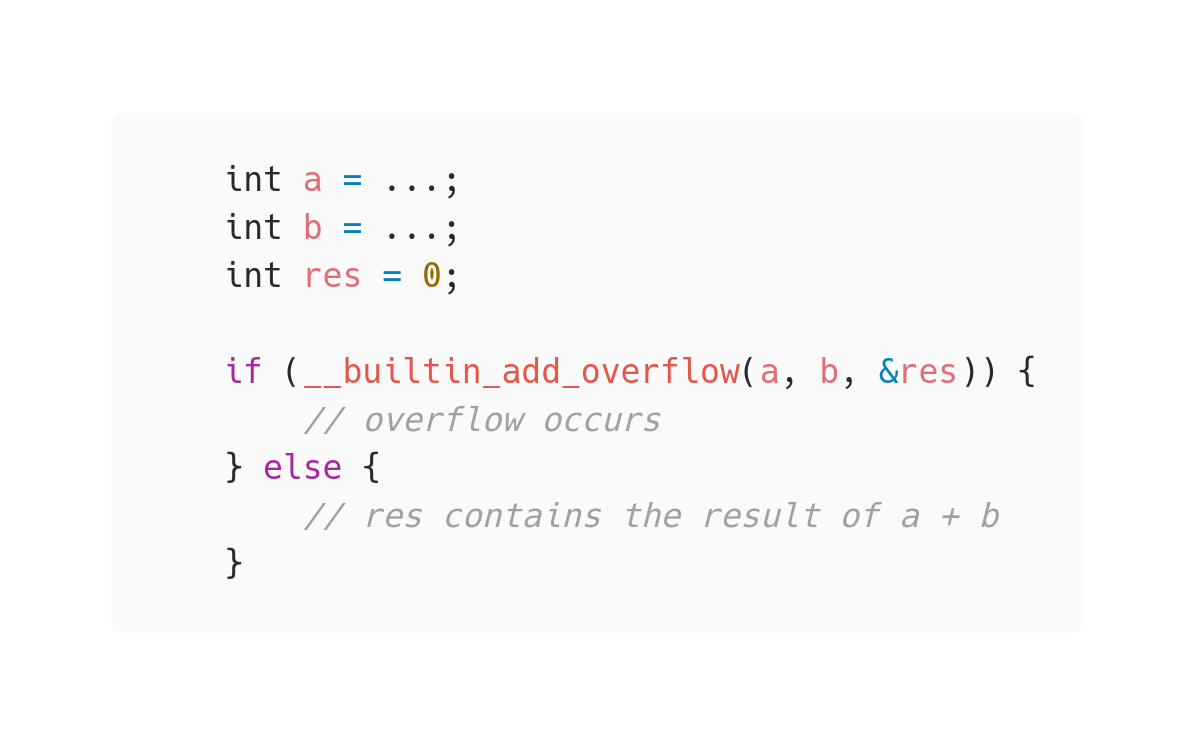
\includegraphics[width=200px]{bultin_add_overflow.png}
\end{frame}

\begin{frame}
    \center\huge{Ввод-вывод в С}
\end{frame}

\begin{frame}
    \center{\textbf{Текстовый поток} — это последовательность символов, разбитая на строки, каждая из которых содержит ноль или более символов и завершается символом новой строки. Обязанность следить за тем, чтобы любой поток ввода-вывода отвечал этой модели, возложена на библиотеку: программист, пользуясь библиотекой, не должен заботиться о том, в каком виде строки представляются вне программы}
\end{frame}

\begin{frame}{Про признак окончания строки}
    \begin{itemize}
        \item Разный под разными платформами
        \item \lstinline{\\n} — Unix
        \item \lstinline{\\r} — Mac
        \item \lstinline{\\r\\n} — Windows
    \end{itemize}
\end{frame}

\begin{frame}{Про непотребства в терминале}
    \begin{itemize}
        \item \lstinline{\\r} переводит каретку в начало строки, но не переносит саму строку
        \item Существуют специальные последовательности символов, которые изменяют состояние терминала
        \item Можно менять позицию курсора, цвет символов, цвет фона и даже издавать звук!
    \end{itemize}
\end{frame}

\begin{frame}
    \center\huge{\textcolor{red}{П}\textcolor{orange}{о}\textcolor{yellow}{р}\textcolor{green}{и}\textcolor{blue}{с}\textcolor{magenta}{у}\textcolor{red}{е}\textcolor{orange}{м}
\textcolor{yellow}{в}
\textcolor{green}{т}\textcolor{blue}{е}\textcolor{magenta}{р}\textcolor{red}{м}\textcolor{orange}{и}\textcolor{yellow}{н}\textcolor{green}{а}\textcolor{blue}{л}\textcolor{magenta}{е}\textcolor{red}{!}}
\end{frame}

\begin{frame}{Про escape sequences}
    \center\qrcode[hyperlink,height=75px]{http://www.lihaoyi.com/post/BuildyourownCommandLinewithANSIescapecodes.html}
\end{frame}

\begin{frame}{Преимущества стандартной библиотеки С}
    \begin{itemize}
        \item Функции стандартной библиотеки С легко вызвать из других языков (например, из ассемблера)
        \item Стандартный ввод-вывод С по умолчанию thread-safe
        \item Стандартный ввод-вывод С (иногда существенно) быстрее
        \item Форматный ввод-вывод С, несмотря на особенности, может оказаться удобнее в использовании
    \end{itemize}
\end{frame}

\begin{frame}
    \center\huge{Вычеркните лишнее}
\end{frame}

\begin{frame}{Вычеркните лишнее}
    \begin{itemize}
        \item Функции стандартной библиотеки С легко вызвать из других языков (например, из ассемблера)
        \item Стандартный ввод-вывод С по умолчанию thread-safe
        \item Стандартный ввод-вывод С (иногда существенно) быстрее
        \item Форматный ввод-вывод С, несмотря на особенности, может оказаться удобнее в использовании
    \end{itemize}
\end{frame}

\begin{frame}{Вычеркните лишнее}
    \begin{itemize}
        \item Функции стандартной библиотеки С легко вызвать из других языков (например, из ассемблера)
        \item Стандартный ввод-вывод С по умолчанию thread-safe
        \item \sout{\textcolor{gray}{Стандартный ввод-вывод С (иногда существенно) быстрее}}
        \item Форматный ввод-вывод С, несмотря на особенности, может оказаться удобнее в использовании
    \end{itemize}
\end{frame}

\begin{frame}{Если когда-то понадобится ускорить C++}
    \begin{itemize}
        \item \lstinline{ios_base::sync_with_stdio(false)}
        \item \lstinline{cin.tie(nullptr)}
    \end{itemize}
\end{frame}

\begin{frame}{}
    \begin{center}
        \Huge{Thanks!}
    \end{center}
\end{frame}

\end{document}
